\documentclass{article}
\usepackage{amsmath}
\usepackage{amsfonts}
\usepackage{amssymb}
\usepackage{mathtools}
\usepackage{tcolorbox}
\usepackage[inline]{enumitem}
\usepackage[a4paper,margin=1in]{geometry}
\usepackage[normalem]{ulem}
\usepackage{graphicx}
\usepackage{tasks}
\settasks{label=(\alph*), label-offset=0.4em, label-width=1.5em}

\usepackage{fancyhdr}
\fancyhf{}
\setlength{\headheight}{36pt}
\renewcommand{\headrulewidth}{0pt}
\thispagestyle{fancy}
\lhead{Calculus Exercise}
\chead{Week 15 (9.5, 10.1, 10.2)}
\rhead{\underline{ID:\hspace{7.4em}} \\ \vspace{0.2cm} \underline{Name:\hspace{6em}}}
\cfoot{\thepage}

\begin{document}
\begin{enumerate}
\item[9.5.30]
    Solve the second-order equation $xy'' + 2y' = 12x^2$ by making the substitution $u=y'$.

    \vspace{5cm}

\item[9.5.35]
    Let $P(t)$ be the performance level of someone learning a skill as a function
    of the training time $t$. The graph of $P$ is called a learning curve.
    In Exercise 9.1.27 we proposed the differential equation
    \[\frac{dP}{dt} = k[M - P(t)]\]
    as a reasonable model for learning, where $k$ is a positive constant.
    Solve it as a linear differential equation and use your solution to graph the learning curve.

    \vspace{5cm}

\item[9.5.41]
    \begin{enumerate}
        \item Show that the substitution $z = 1/P$ transforms the logistic differential
            equation $P' = kP(1 - P/M)$ into the linear differential equation \[ z' + kz = \frac{k}{M}\]
        \item Solve the linear differential equation in part (a) and thus obtain
            an expression for $P(t)$. Compare with the following equation.
            \[
                P(t) = \frac{M}{1+A e^{-kt}} \text{, where }
                A = \frac{M - P_0}{P_0}.
            \]
    \end{enumerate}

    \newpage

\item[10.1.30]
    Match each pair of graphs of equations $x=f(t)$, $y=g(t)$ in (a)-(d) with one of
    the parametric curves $x=f(t)$, $y=g(t)$ labeled I–IV. Give reasons for your choices.

    \begin{figure}[h]
        \centering
        \begin{minipage}{.5\textwidth}
            \centering
            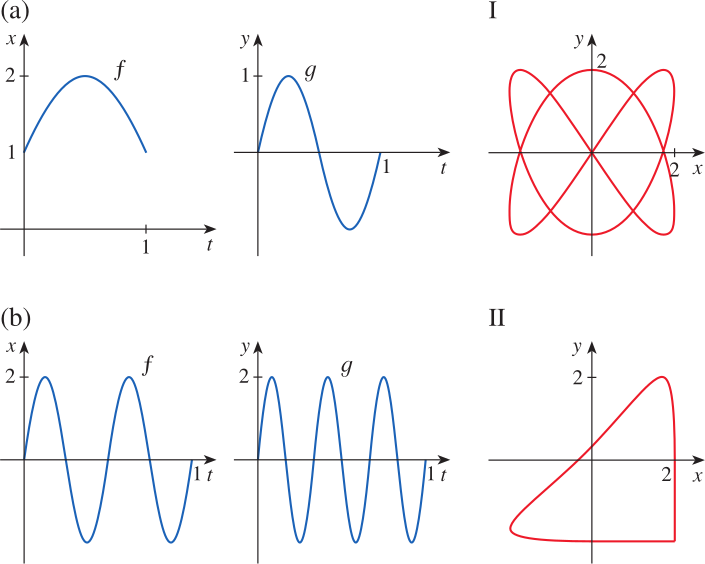
\includegraphics[width=.8\linewidth]{./png/10.1.30.png}
        \end{minipage}%
        \begin{minipage}{.5\textwidth}
            \centering
            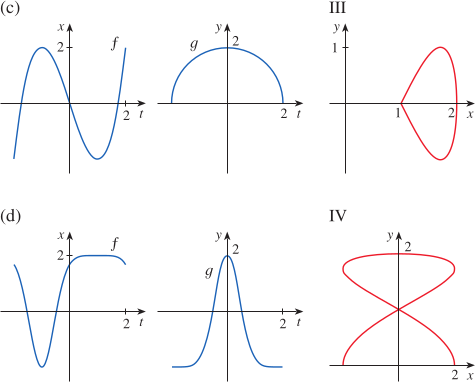
\includegraphics[width=.8\linewidth]{./png/10.1.30-2.png}
        \end{minipage}
    \end{figure}

    \vspace{6cm}

\item[10.1.49]
    Let $P$ be a point at a distance $d$ from the center of a circle of radius $r$.
    The curve traced out by $P$ as the circle rolls along a straight line is called
    a \textbf{trochoid}.
    (Think of the motion of a point on a spoke of a bicycle wheel.)
    The cycloid is the special case of a trochoid with $d=r$.
    Using the same parameter $\theta$ as for the cycloid, and assuming the line is
    the x-axis and $\theta=0$ when $P$ is at one of its lowest points,
    show that parametric equations of the trochoid are
    \[ x=r\theta-d\sin{\theta} \qquad y=r-d\cos{\theta}\]
    Sketch the trochoid for the cases $d<r$ and $d>r$.

    \newpage

\item[10.1.53]
    A curve, called a \textbf{witch of Maria Agnesi}, consists of all possible
    positions of the point $P$ in the figure. Show that parametric
    equations for this curve can be written as
    \[x=2a\cot{\theta},\ y=2a\sin^{2}{\theta}\]
    Sketch the curve.

    \begin{center}
        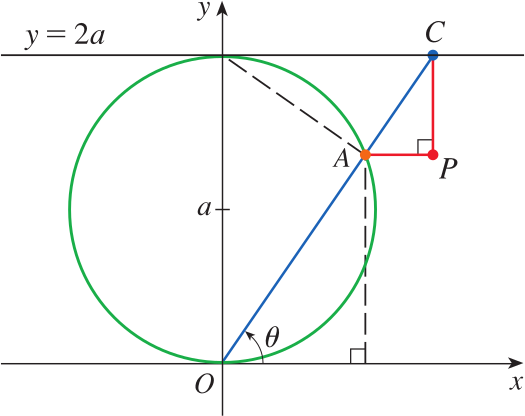
\includegraphics[height=4cm]{./png/10.1.53.png}
    \end{center}

\vspace{4cm}

\item[10.2.18]
    Find $dy/dx$ and $d^{2}y/dx^{2}$. For which values of $t$ is the curve concave upward?
    \[x=t^2+1,\ y=e^{t}-1\]

\vspace{4cm}

\item[10.2.31]
    \begin{enumerate}
        \item Find the slope of the tangent line to the trochoid $x=r\theta-d\sin{\theta}$,
            $y=r-d\cos{\theta}$ in term of $\theta$. (See Exercise 10.1.49).
        \item Show that if $d < r$, then the trochoid does not have a vertical tangent.
    \end{enumerate}

\newpage

\item[10.2.38]
    Find the area enclosed by the given parametric curve and the $y$-axis.
    \[x = t^2 - 2t ,\ y=\sqrt{t}\]

    \begin{center}
        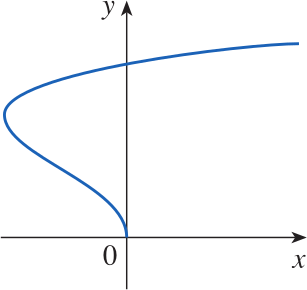
\includegraphics[height=4cm]{./png/10.2.38.png}
    \end{center}

\vspace{4cm}

\item[10.2.50]
    Find the exact length of the curve. \[x=3\cos{t}-\cos{3t}, \qquad y=3\sin{t}-\sin{3t}, \qquad 0 \leqslant t \leqslant \pi\]

\vspace{5cm}

\item[10.2.73]
    Find the exact area of the surface obtained by rotating the given curve about the $x$-axis.
    \[x=a\cos^{3}{\theta}, \qquad y=a\sin^{3}{\theta}, \qquad 0 \leqslant \theta \leqslant \pi/2\]

\end{enumerate}
\end{document}
